\documentclass[journal,12pt,twocolumn]{IEEEtran}
\usepackage{romannum}
\usepackage{float}
\usepackage{setspace}
\usepackage{gensymb}
\singlespacing
\usepackage[cmex10]{amsmath}
\usepackage{amsthm}
\usepackage{mathrsfs}
\usepackage{txfonts}
\usepackage{stfloats}
\usepackage{bm}
\usepackage{cite}
\usepackage{cases}
\usepackage{subfig}
\usepackage{longtable}
\usepackage{multirow}
\usepackage{enumitem}
\usepackage{mathtools}
\usepackage{steinmetz}
\usepackage{tikz}
\usepackage{circuitikz}
\usepackage{verbatim}
\usepackage{tfrupee}
\usepackage[breaklinks=true]{hyperref}
\usepackage{tkz-euclide}
\usetikzlibrary{calc,math}
\usepackage{listings}
    \usepackage{color}                                            %%
    \usepackage{array}                                            %%
    \usepackage{longtable}                                        %%
    \usepackage{calc}                                             %%
    \usepackage{multirow}                                         %%
    \usepackage{hhline}                                           %%
    \usepackage{ifthen}                                           %%
  %optionally (for landscape tables embedded in another document): %%
    \usepackage{lscape}     
\usepackage{multicol}
\usepackage{chngcntr}
\DeclareMathOperator*{\Res}{Res}
\renewcommand\thesection{\arabic{section}}
\renewcommand\thesubsection{\thesection.\arabic{subsection}}
\renewcommand\thesubsubsection{\thesubsection.\arabic{subsubsection}}

\renewcommand\thesectiondis{\arabic{section}}
\renewcommand\thesubsectiondis{\thesectiondis.\arabic{subsection}}
\renewcommand\thesubsubsectiondis{\thesubsectiondis.\arabic{subsubsection}}

% correct bad hyphenation here
\hyphenation{op-tical net-works semi-conduc-tor}
\def\inputGnumericTable{}                                 %%

\lstset{
frame=single, 
breaklines=true,
columns=fullflexible
}

\begin{document}


\newtheorem{theorem}{Theorem}[section]
\newtheorem{problem}{Problem}
\newtheorem{proposition}{Proposition}[section]
\newtheorem{lemma}{Lemma}[section]
\newtheorem{corollary}[theorem]{Corollary}
\newtheorem{example}{Example}[section]
\newtheorem{definition}[problem]{Definition}
\newcommand{\BEQA}{\begin{eqnarray}}
\newcommand{\EEQA}{\end{eqnarray}}
\newcommand{\define}{\stackrel{\triangle}{=}}

\bibliographystyle{IEEEtran}
\providecommand{\mbf}{\mathbf}
\providecommand{\pr}[1]{\ensuremath{\Pr\left(#1\right)}}
\providecommand{\qfunc}[1]{\ensuremath{Q\left(#1\right)}}
\providecommand{\sbrak}[1]{\ensuremath{{}\left[#1\right]}}
\providecommand{\lsbrak}[1]{\ensuremath{{}\left[#1\right.}}
\providecommand{\rsbrak}[1]{\ensuremath{{}\left.#1\right]}}
\providecommand{\brak}[1]{\ensuremath{\left(#1\right)}}
\providecommand{\lbrak}[1]{\ensuremath{\left(#1\right.}}
\providecommand{\rbrak}[1]{\ensuremath{\left.#1\right)}}
\providecommand{\cbrak}[1]{\ensuremath{\left\{#1\right\}}}
\providecommand{\lcbrak}[1]{\ensuremath{\left\{#1\right.}}
\providecommand{\rcbrak}[1]{\ensuremath{\left.#1\right\}}}
\theoremstyle{remark}
\newtheorem{rem}{Remark}
\newcommand{\sgn}{\mathop{\mathrm{sgn}}}
\providecommand{\abs}[1]{\left\vert#1\right\vert}
\providecommand{\res}[1]{\Res\displaylimits_{#1}} 
\providecommand{\norm}[1]{\left\lVert#1\right\rVert}
\providecommand{\mtx}[1]{\mathbf{#1}}
\providecommand{\mean}[1]{E\left[ #1 \right]}
\providecommand{\fourier}{\overset{\mathcal{F}}{ \rightleftharpoons}}
\providecommand{\system}{\overset{\mathcal{H}}{ \longleftrightarrow}}
\newcommand{\solution}{\noindent \textbf{Solution: }}
\newcommand{\cosec}{\,\text{cosec}\,}
\providecommand{\dec}[2]{\ensuremath{\overset{#1}{\underset{#2}{\gtrless}}}}
\newcommand{\myvec}[1]{\ensuremath{\begin{pmatrix}#1\end{pmatrix}}}
\newcommand{\mydet}[1]{\ensuremath{\begin{vmatrix}#1\end{vmatrix}}}
\numberwithin{equation}{subsection}
\makeatletter
\@addtoreset{figure}{problem}
\makeatother

\let\StandardTheFigure\thefigure
\let\vec\mathbf
\renewcommand{\thefigure}{\theproblem}



\def\putbox#1#2#3{\makebox[0in][l]{\makebox[#1][l]{}\raisebox{\baselineskip}[0in][0in]{\raisebox{#2}[0in][0in]{#3}}}}
     \def\rightbox#1{\makebox[0in][r]{#1}}
     \def\centbox#1{\makebox[0in]{#1}}
     \def\topbox#1{\raisebox{-\baselineskip}[0in][0in]{#1}}
     \def\midbox#1{\raisebox{-0.5\baselineskip}[0in][0in]{#1}}

\vspace{3cm}


\title{Assignment 1}
\author{Jaswanth Chowdary Madala}





% make the title area
\maketitle

\newpage

%\tableofcontents

\bigskip

\renewcommand{\thefigure}{\theenumi}
\renewcommand{\thetable}{\theenumi}



\begin{enumerate}
\item A dietician has to develop a special diet using two foods $P$ and $Q$. Each packet (containing 30 g) of food $P$ contains 12 units of calcium, 4 units of iron, 6 units of cholesterol and 6 units of vitamin A. Each packet of the same quantity of food $Q$ contains 3 units of calcium, 20 units of iron, 4 units of cholesterol and 3 units of vitamin A. The diet requires atleast 240 units of calcium, atleast 460 units of iron and at most 300 units of cholesterol. How many packets of each food should be used to maximise the amount of vitamin A in the diet? What is the maximum amount of vitamin A in the diet?\\
\textbf{Solution:} Let $x$ and $y$ be the number of packets of food $P$ and $Q$ respectively
\begin{align}
x &\geq 0 \label{eq:1}\\
y &\geq 0 \label{eq:2}
\end{align}
From the constraint on Calcium we have,
\begin{align}
12x + 3y &\geq 240 \\
\implies 4x+y &\geq 80\label{eq:3}
\end{align}
From the constraint on Iron we have,
\begin{align}
4x + 20y &\geq 460 \\
\implies x+5y &\geq 115\label{eq:4}
\end{align}
From the constraint on cholesterol we have,
\begin{align}
6x + 4y &\leq 300\\
\implies 3x+2y &\leq 150 \label{eq:5}
\end{align}
Vitamin A in the diet is given by,
\begin{align}
Z = 6x + 3y
\end{align}

\begin{enumerate}
\item Using cvxpy method: The given problem can be formulated as,
\begin{align}
\min_{\vec{x}} -Z &= \myvec{-6 & -3}\vec{x} \\
\text{s.t.} \quad \vec{A}\vec{x} &\leq B
\end{align}
where
\begin{align}
A &= \myvec{-1&0 \\ 0&-1 \\ -4&-1 \\ -1&-5 \\ 3&2}\\
B &= \myvec{0\\0\\-80\\-115\\150}
\end{align}
By solving using cvxpy, we get
\begin{align}
\max_{\vec{x}} Z &= 285 \\
\vec{x} &= \myvec{40 \\15} 
\end{align}
\item Using Corner point method: The corner points of the inequalities are:
\begin{align}
\vec{P} &= \myvec{2 \\ 72}\\
\vec{Q} &= \myvec{15 \\ 20}\\
\vec{R} &= \myvec{40 \\ 15}
\end{align}
We have
\begin{align}
Z = – 3x + 4 y \label{eq:6}
\end{align}
Substituting above values of corner points in Equation \eqref{eq:6} to get the value of $Z$, as shown in the table \ref{tab:1}
\begin{table}[h]
\centering
%%%%%%%%%%%%%%%%%%%%%%%%%%%%%%%%%%%%%%%%%%%%%%%%%%%%%%%%%%%%%%%%%%%%%%
%%                                                                  %%
%%  This is a LaTeX2e table fragment exported from Gnumeric.        %%
%%                                                                  %%
%%%%%%%%%%%%%%%%%%%%%%%%%%%%%%%%%%%%%%%%%%%%%%%%%%%%%%%%%%%%%%%%%%%%%%

\begin{center}
\begin{tabular}{|c|c|c|}
\hline
\textbf{RV}& \textbf{Values} & \textbf{Description} \\ \hline
$X$		   & 	$\{0,1\}$	&  1st draw - 0: black card, 1: red card\\ \hline
$Y$ 		   & 	$\{0,1\}$	&  2nd draw - 0: black card, 1: red card\\ \hline
$X,Y$ 		   & 	$\{00\}$	&	2 cards drawn are black\\ \hline
\end{tabular}
\end{center}

\caption{}
\label{tab:1}
\end{table}
From the table \ref{tab:1}, the optimum point and optimum value are 
\begin{align}
\vec{R} &=\myvec{4\\0}\\
\max Z &= 285
\end{align}
\begin{figure}[ht]
\centering
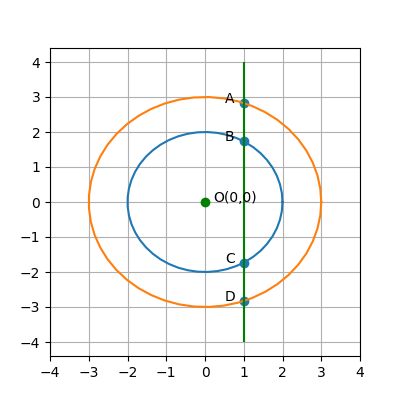
\includegraphics[width = \columnwidth]{"figs/fig.png"}
\caption{Graph}
\label{fig:1}
\end{figure}

\end{enumerate}
\end{enumerate}
\end{document}


